\chapter{Toy examples and experiments}

\section{Minimal example?}

\section{Points on the line}

The first example we present is a selection of points on a (discretised) line. More precisely we will assume that we have \(100\) points on a line that are equally spaced and we aim to model a spacial repulsion between the selected points. For this we will use the method \ref{moddiv} of reference points % \todo{formulate and cite it!} of modelling
 the diversity features. In this case we will use the set \(\mathcal Y\) itself as reference set and use a 

\begin{emp}[Setup of the example]
Let \(\mathcal Y \coloneqq\left\{ 1, \dots, 100\right\}\) and for \(i\in\mathcal Y\). Then we will  let \(\phi_i\in\mathbb R^{100}\) be given up to scaling by
\[(\phi_i)_j\propto f\left(\frac{\left\lvert i - j \right\rvert}{???}\right)\]
where \(f\) is the density of the standard nomal distribution. Further we choose the qualities to be constant and so that the expected cardinatlity is \(10\)\todo{check}.
\end{emp}

\begin{rem}%[Remark]
\begin{enumerate}
\item describe scaling including choice of cardinality
\item describe rank of the kernel?
\item describe choice of �repulsiveness�, plot density around a point; make comment to kernel methods? comment on the qualitative properties of \(f\) and why they are suitable here
\end{enumerate}
% \todo{explain scaling of the quality}
\end{rem}

To make the difference to an uncorrelated point pattern more apparent we also defined a Poisson process, i.e. a DPP without correlations between the points with the same expected cardinality. The sampling results are compared in Figure \ref{fig:4.1}.% Such uncorrelated DPPs are called \emph{Poisson point processes}.\todo{introduce earlier!}

\vspace{2cm}
\begin{figure}[h!]
	\centering
	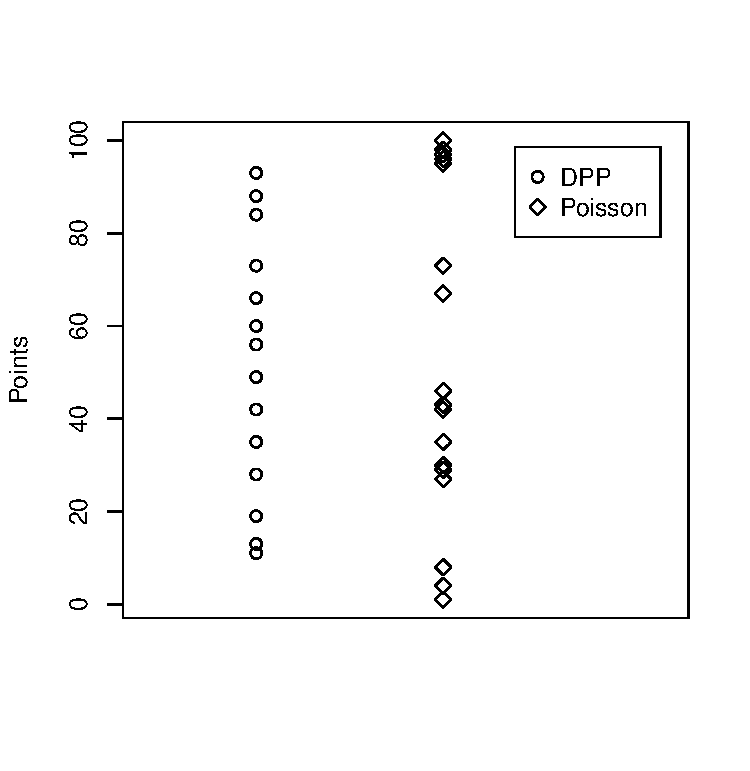
\includegraphics[width=0.6\textwidth]{comparison-dpp-poisson}
%	\tag{1}
	\caption{Comparison of a DPP with negative correlations on the left and no correlations, i.e. a Poisson point process on the right.}
	\label{fig:4.1}
\end{figure}
\todo{make comment on zeta function!}

\begin{emp}[Representation as binary sequence]

\end{emp}
\todo{comment on problems and findings?}
\section{Points in the square}

\section{Toy example for quality learning}